\documentclass[10pt]{beamer}
\usetheme[progressbar=frametitle]{metropolis}
\usepackage{amsmath}
\usepackage{amsfonts}
\usepackage{commath}
\usepackage{mathtools}
\usepackage{tabu}
\usepackage{booktabs}
\usepackage{bm}
\usepackage{xfrac}
\usepackage{subcaption}
\usepackage{graphicx}
\usepackage{pgfplots}
\usepackage{hyperref}
\hypersetup{pdfpagemode=FullScreen}

\newcommand{\RR}{\mathbb{R}}
\DeclarePairedDelimiter\ip{\langle }{\rangle}

\title{Diff Geo}
\subtitle{Gyroscopic Data Analysis Using SO(3)}
\date{\today}
\author{Nick Draper \and Jonathan Hayase}
\institute{Math 143 -- Differential Geometry Seminar -- Spring 2018}

\begin{document}

\maketitle

\begin{frame}{Table of contents}
    \setbeamertemplate{section in toc}[sections numbered]
    \tableofcontents[hideallsubsections]
\end{frame}

\section{Introduction}

\begin{frame}
Typical devices will usually contain a multitude of sensors for measuring properties that can be useful for modeling and analysis such as accelerations, rotational velocities, and magnetic fields just to name a few. 
\begin{figure}
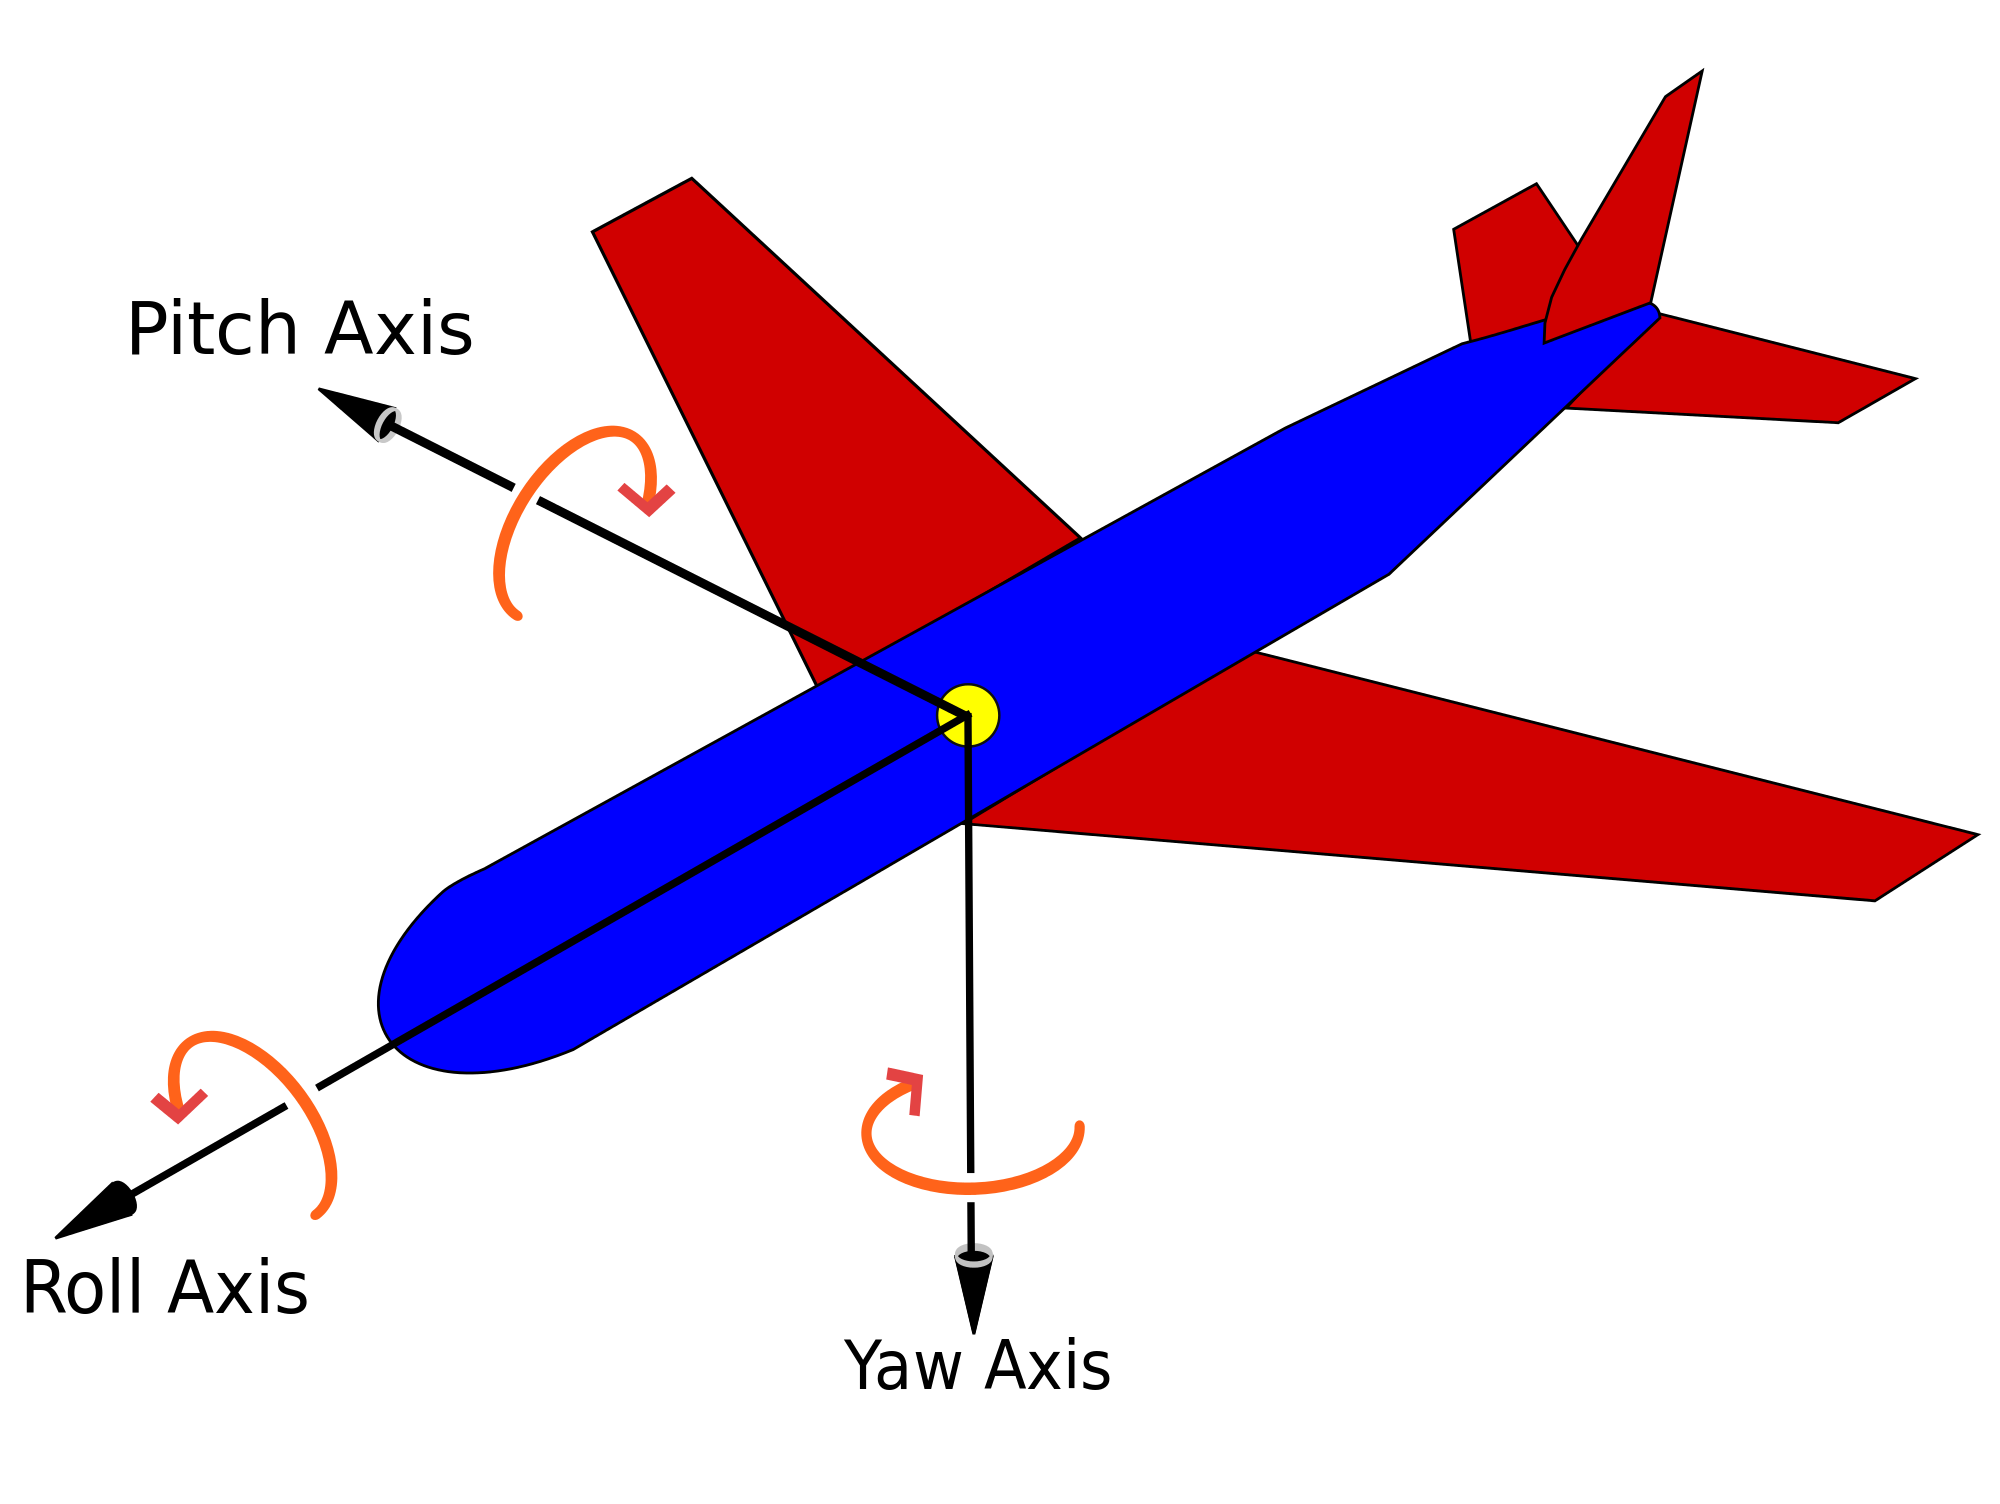
\includegraphics[scale=0.08]{images/plane.png}
\caption{Illustration of a plane with its corresponding axes of rotation labeled \cite{plane1}.}
\end{figure}
\end{frame}

\begin{frame}
We can capture such data from Android  cellphones and try to mathematically find patterns of what people are doing with their phone. 
\end{frame}

\section{Dataset}

\begin{frame}
We will be using the hand movement, orientation, and
grasp (HMOG) dataset \cite{phone}. This dataset contains a set of behavioral  
\end{frame}

\section{Error Sources}

\begin{frame}
Assuming we have perfect uniform time sampled data, there are still a number of errors that can appear in the data.
\begin{enumerate}
\item Bias
\item White Noise
\item Temperature Effects
\item Calibration
\item Bias Instability
\end{enumerate}
\end{frame}

\begin{frame}
\frametitle{Bias Error}
Bias is some marginal error $\epsilon$ that is incorporated when we try to integrate the data. The error is proportional to the time interval we integrate over.
\begin{equation*}
\theta(t) = \epsilon \cdot t
\end{equation*}
\end{frame}

\begin{frame}
\frametitle{White Noise Error}
White noise is a type of noise that has an associated standard deviation of $\sigma$. As we integrate this error is grows proportionally with the square root of time. 
\begin{equation*}
\sigma_{\theta}(t) = \sigma \cdot \sqrt{\partial t \cdot t}
\end{equation*}
\end{frame}

\begin{frame}
\frametitle{Temperature Effect Error}
Residual bias that depends on temperature. This residual bias is factored into the orientation which causes an error in the orientation data. This error is proportional with time.
\end{frame}

\begin{frame}
\frametitle{Calibration Error}
Calibration errors can be attributed to errors in the scale factors, alignments, and the gyro linearities. When integrating this kind of error, it is proportional to the rate and duration of motion.
\end{frame}

\begin{frame}
\frametitle{Bias Instability Error}
This kind of error can be attributed to bias fluctuations and can be modeled as a bias random walk. When integrating this kind of error, it results in a second-order random walk.  
\end{frame}

\begin{frame}
\frametitle{References}
\bibliographystyle{plain}
\bibliography{references}
\end{frame}

\end{document}
